\documentclass[a4paper,12pt]{report}  
\usepackage{xcolor}
\usepackage{graphicx}
\graphicspath{ {./code_snaps/} }

\begin{document}
\chapter{\bf{METHODOLOGY and MODEL EQUATION}}

\begin{figure}
\section{\bf Coding Implementation}\vspace{1cm}
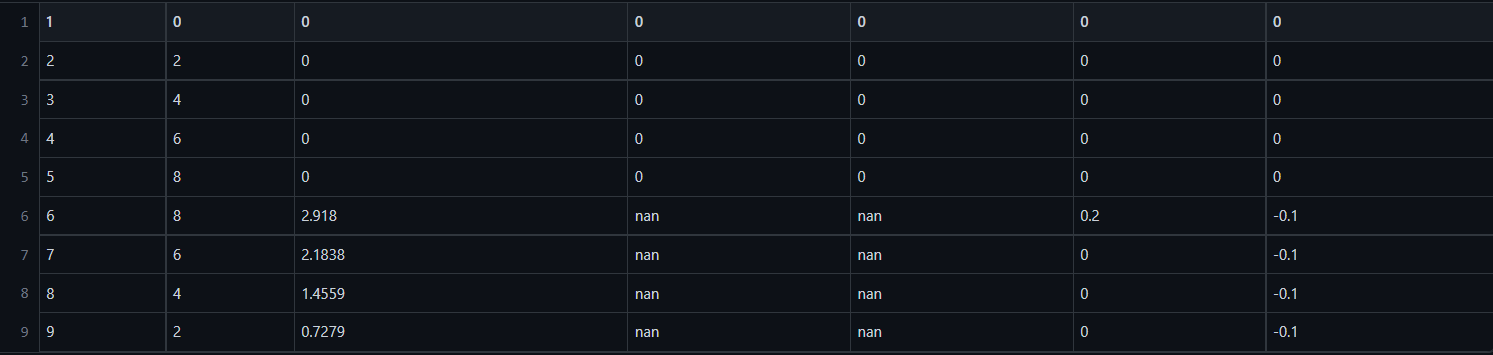
\includegraphics[width=14cm, height=4cm]{node}
\caption{node.csv}
\vspace{0.7cm}
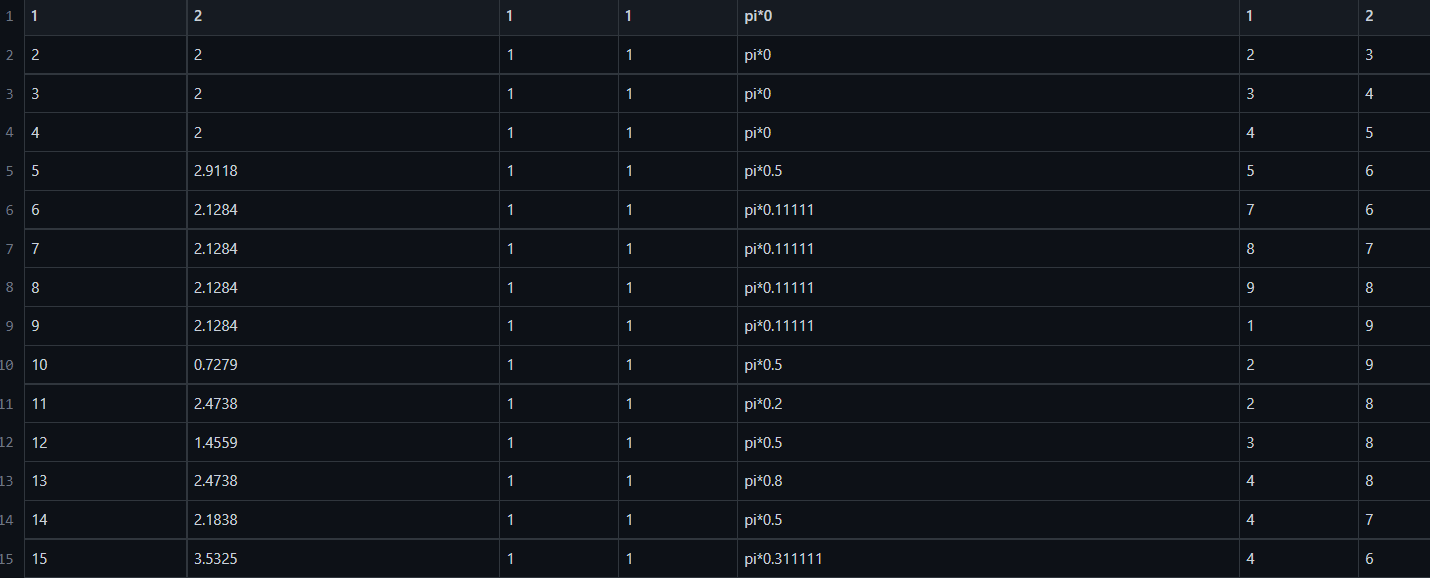
\includegraphics[width = 14cm, height = 6cm]{ele}
\caption{element.csv}
\vspace{0.7cm}
To feed the data to our program, we came up with the idea of using csv files so as to make the program available for general problems and for a easy to input interface.\\

Figure 1.1 shows the input format of nodes where each row represents a node and its attribues: node number, position on x and y-axis, its displacement on x and y-axis and the force applied on x and y-axis.\\

Similarly, Figure 1.2 shows the input format of the elements where each row represents a element and its attribues: element number, length , cross-section area , young's modulus , angle with the global x-axis and the nodes that it connects.
\end{figure}
\begin{figure}
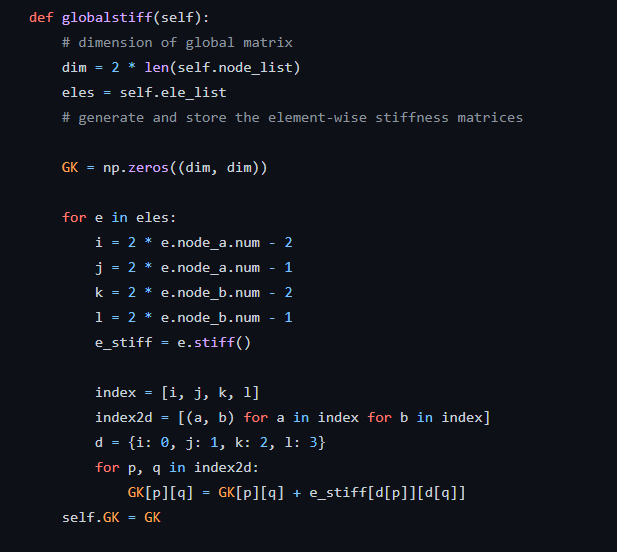
\includegraphics[width = 14cm, height = 11cm]{gm}
\caption{Forming the global stiffness matrix}
\vspace{1cm}
Formation of global stiffness matrix was a challenge and reducing the code to faster execution and simplicity was even bigger of a task. Finally the method applied is shown in the Figure 1.3.\\

\begin{verbatim}
	content...
\end{verbatim}
	
 The list of elements is iterated throughout for accessing each element. Then with the logic of how the values in local stiffness matrix is appended to the global matrix, we came up with an efficient algorithm that fits well to our purpose as well as works on all such general problems with slightest of tweaks.
\end{figure}
\begin{figure}
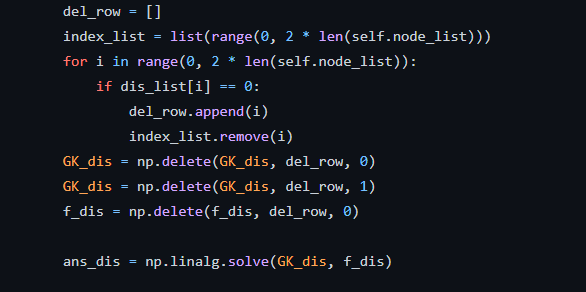
\includegraphics[width = 14cm, height = 8cm]{solve}
\caption{Solution}
\vspace{1cm}

After generating global stiffness matrix we now had 3 variables: the stiffness matrix , the displacement and the force vector. For simplifying the calculations and faster computation, for $n^{th}$ element being 0 in the displacement vector we reduced the global matrix by removing coressponding $n^{th}$ row and columns (Figure 1.4). After reduction simple linear algebra has been applied to find out the unknown/missing values of displacement of each node. 
\end{figure}
\begin{figure}
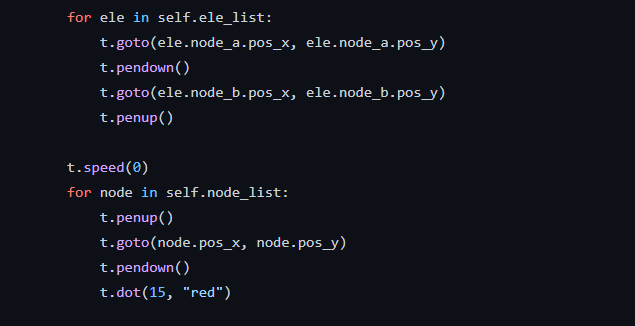
\includegraphics[width = 15cm, height = 8cm]{ini_vis}
\caption{}
\vspace{1cm}
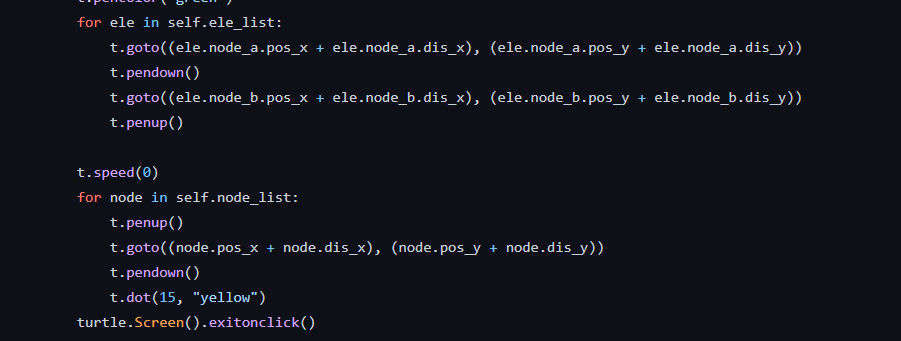
\includegraphics[width = 15cm, height = 7cm]{fin_vis}
\caption{}
\vspace{1cm}

For the last and final part of visualizing our problem and the visualizing the solution so as to make each bit of data understandable we used the Turtle module of Python. Initially we draw our problem provided the position of the nodes and elements connecting them (Figure 1.5). Then from the displacement data of each node we get after the computation, the same algorithm is applied to draw the final result/ shape of the truss. This time the position of node is the sum of its original position and its displacement in x and y-axis (Figure 1.6). Different tools have been used to make the visualized problem and result understandable.
\end{figure}
\end{document}